% Chapter: Client

This chapter explains overall architecture of the \textan{} client application.
It provides description of the most important packages and diagrams illustrating
the structure of this part of the project.

\section{Client Architecture}
\textan{} client consist of two main parts. The package
\emph{cz.cuni.mff.ufal.textan.core} and its subpackages handle communication
with webservices and completely hides them from the package
\emph{cz.cuni.mff.ufal.textan.core} and its subpackages which are responsible
for actual displaying the user interface (see Figure \ref{fig:ClientOverview}).
It means that the model representation is duplicite to classes generated from
the WSDL by CXF into \emph{cz.\-cuni.\-mff.\-ufal.\-textan.\-commons.\-model}
and \emph{cz.\-cuni.\-mff.\-ufal.\-textan.\-commons.\-ws} and their subpackages.
On the other hand this approach has great advantage - webservice interface
changes will require only code refactoring localized into \emph{core.*}
packages. There is also \emph{cz.\-cuni.\-mff.\-ufal.\-textan.\-tui} package
containing a simple batch report processor without user interaction.

\begin{figure}[!htb]
        \centering
        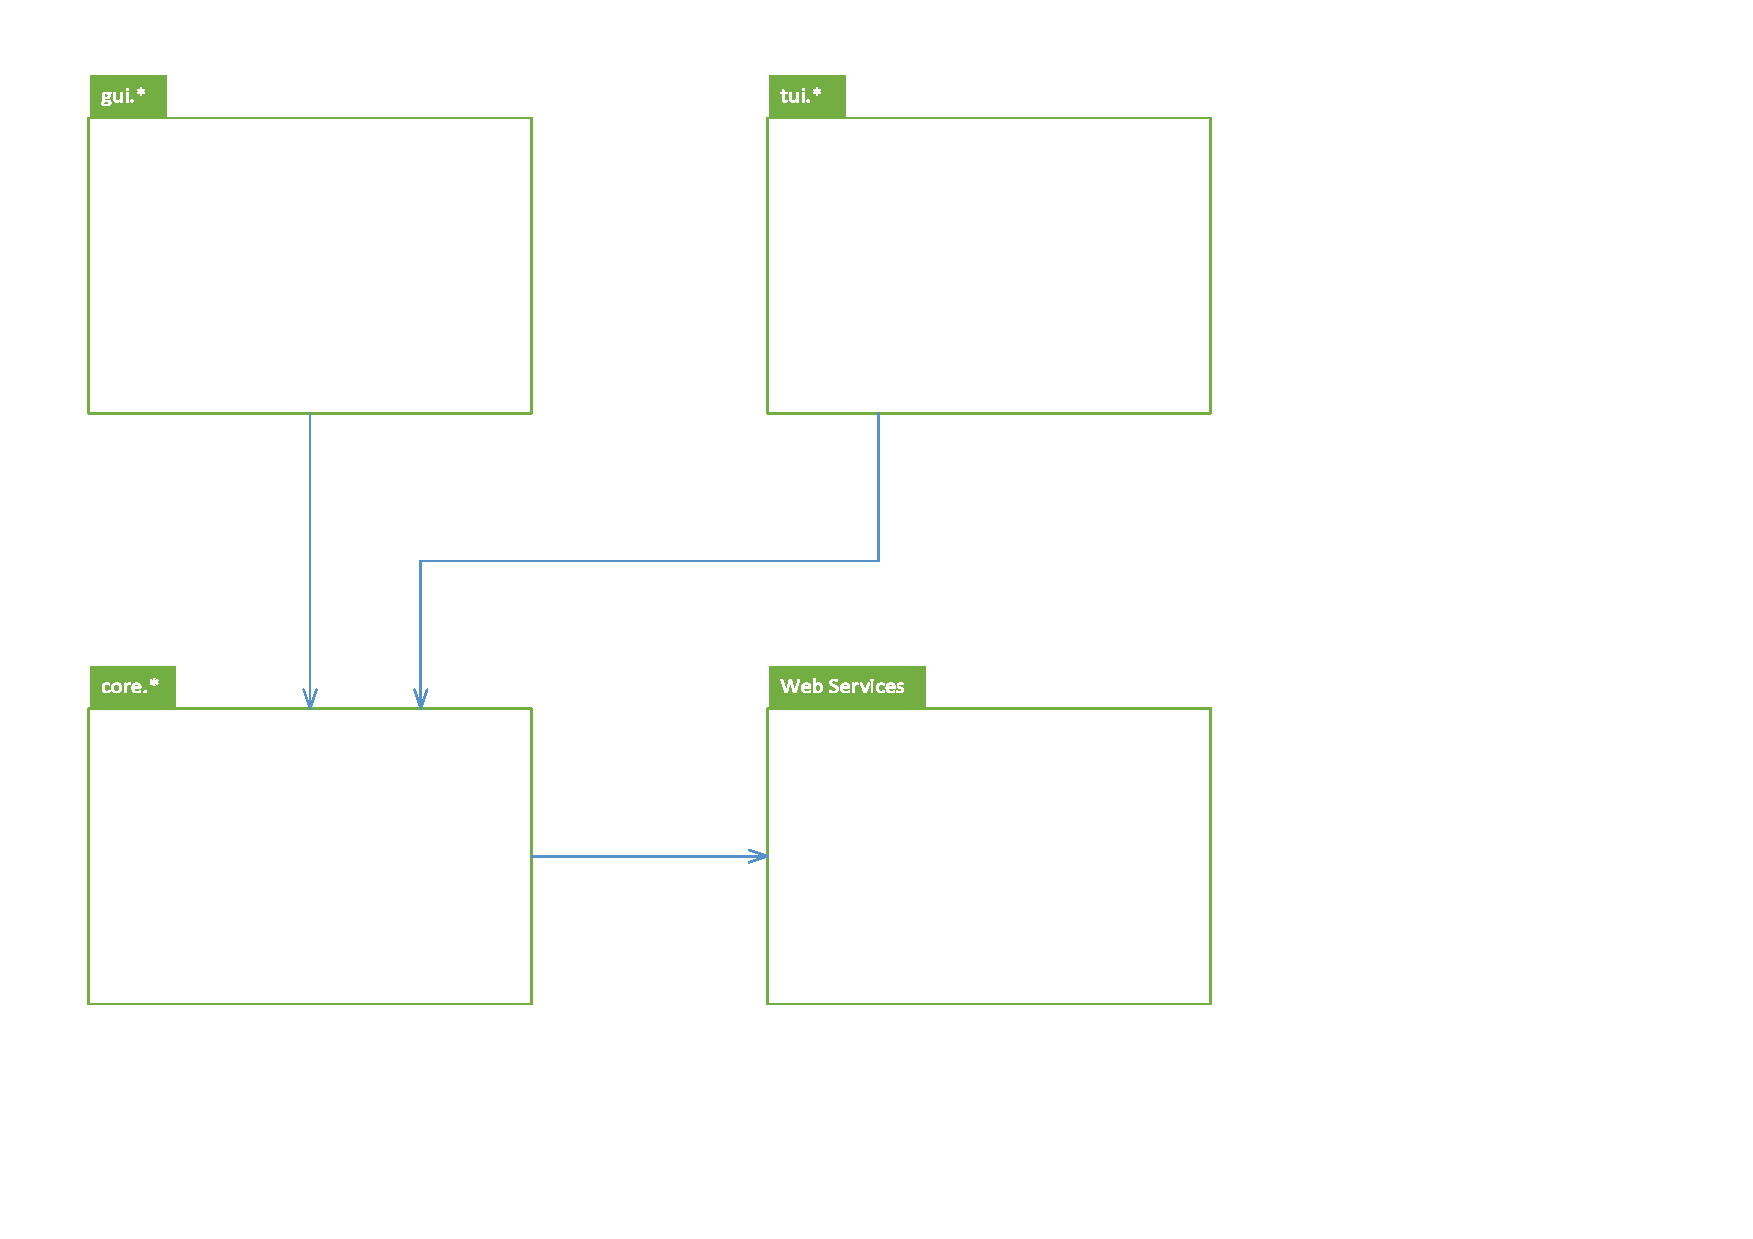
\includegraphics[width=\textwidth]{Images/ClientOverview}
        \caption{Overview of the packages.}
        \label{fig:ClientOverview}
\end{figure}

For visualization itself JavaFX framework is used. It naturally enforces
Model-View-Controller architecture.

In the rest of the section the most important packages will be introduced and
described.

\section{Model - cz.cuni.mff.ufal.textan.core}

Model classes can be found in this package. It contains mainly client side
representation of object, entity, relation, document etc. (see Figure
\ref{fig:CorePackage}). The most important class is \emph{Client} which is used
for communication with the webservices. It also serves as a factory of
\emph{ProcessReportPipeline} (see Figure \ref{sssec:ReportPipeline}). There are
also \emph{SynchronizedDataProvider} and \emph{SynchronizedDocumentProcessor} to
provide synchronization for \emph{IDataProvider} and \emph{IDocumentProcessor}
created by CXF.

Subpackages of the \emph{Core} package focus on individual client side tasks,
like displaying graphs and processing reports in a pipeline.

\begin{figure}[!htb]
        \centering
        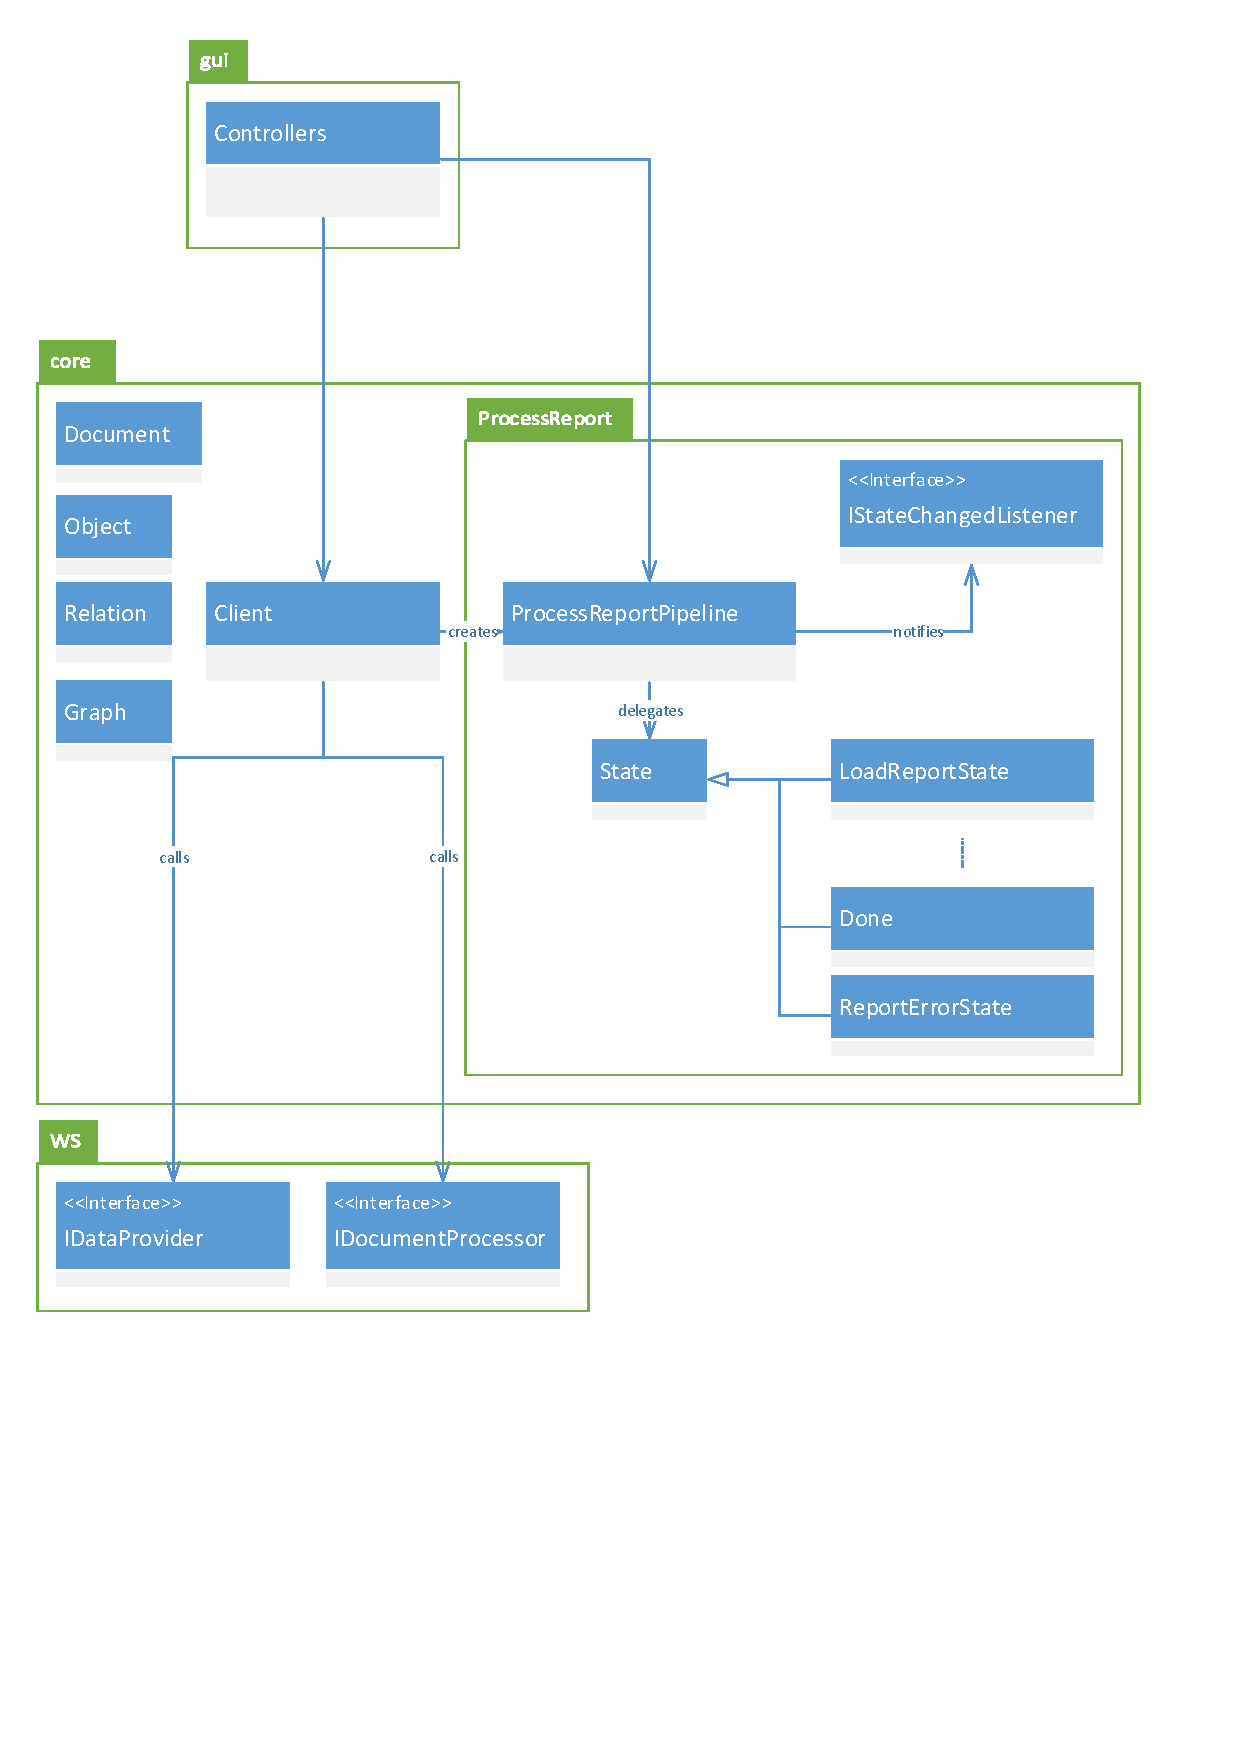
\includegraphics[width=\textwidth]{Images/CorePackage}
        \caption{Overview of the most important features of \emph{core} package.}
        \label{fig:CorePackage}
\end{figure}

\subsection{cz.cuni.mff.ufal.textan.core.reportpipeline}
\label{sssec:ReportPipeline}

This package contains classes necessary for report processing (see Figure
\ref{fig:CorePackage}). Most importantly there is class
\emph{ProcessReportPipeline} that holds information about processing one report.
The pipeline/wizard approach was chosen because the amount of choices and
required tasks would be overwhelming to users if they were all provided at once.
Virtually all methods of the pipeline object are delegated to its \emph{State}
(see figure \ref{fig:Pipeline}). Descendants of the class \emph{State} are
singletons. They contain most of the pipeline processing logic and control to
which state the pipeline should go next. When this happens, each registered
\emph{IStateChangedListener} is notified.

\begin{figure}[!htb]
        \centering
        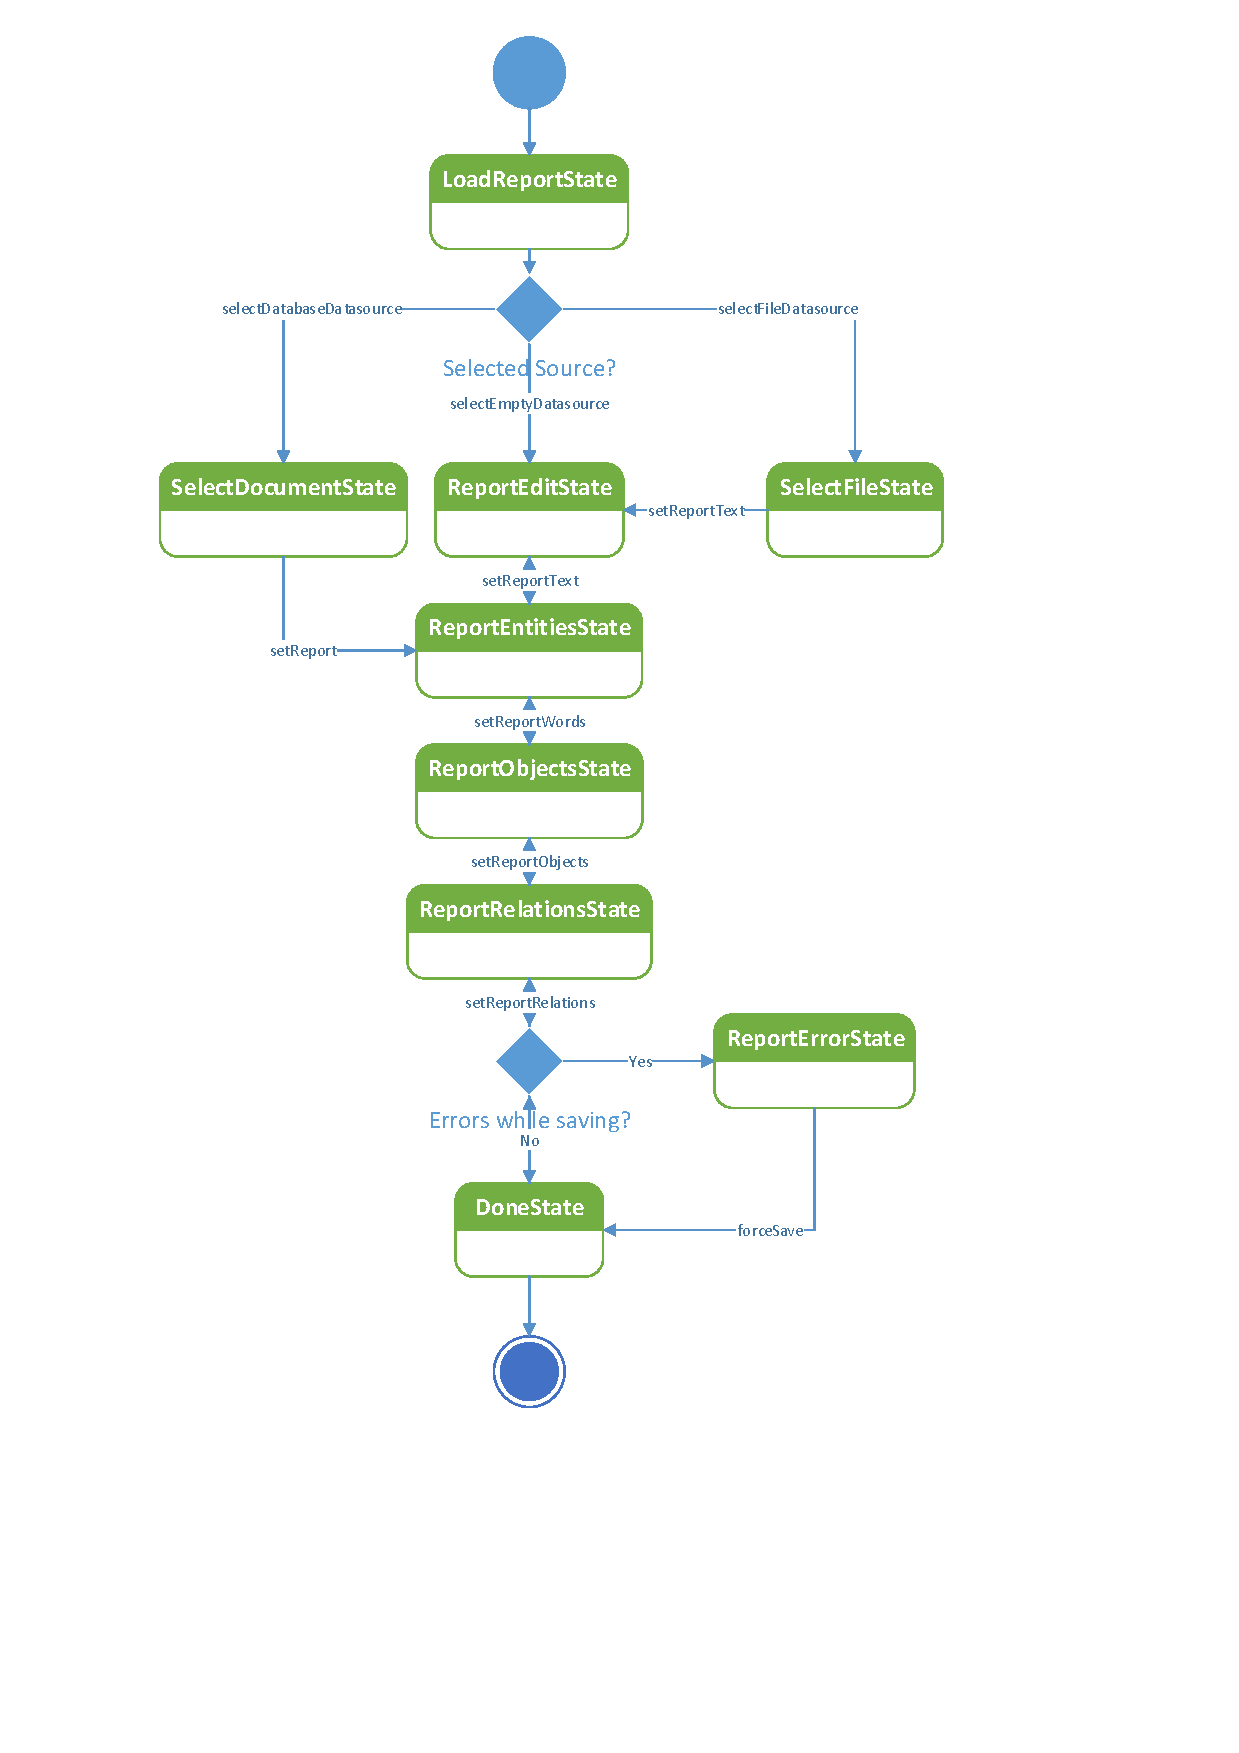
\includegraphics[height=16cm]{Images/Pipeline}
        \caption{Pipeline state machine.}
        \label{fig:Pipeline}
\end{figure}

For easy selecting recognized entities and relations a hierarchy of builders
has been developed (see Figure \ref{fig:Builders}). This is necessary because
\emph{Object} and \emph{Relation} immutable. The \emph{word} is a class
representing independent word of the report text. It can be assigned to either
an entity or relation. \emph{EntityBuilder} also holds the assigned object if
any.

\begin{figure}[!htb]
        \centering
        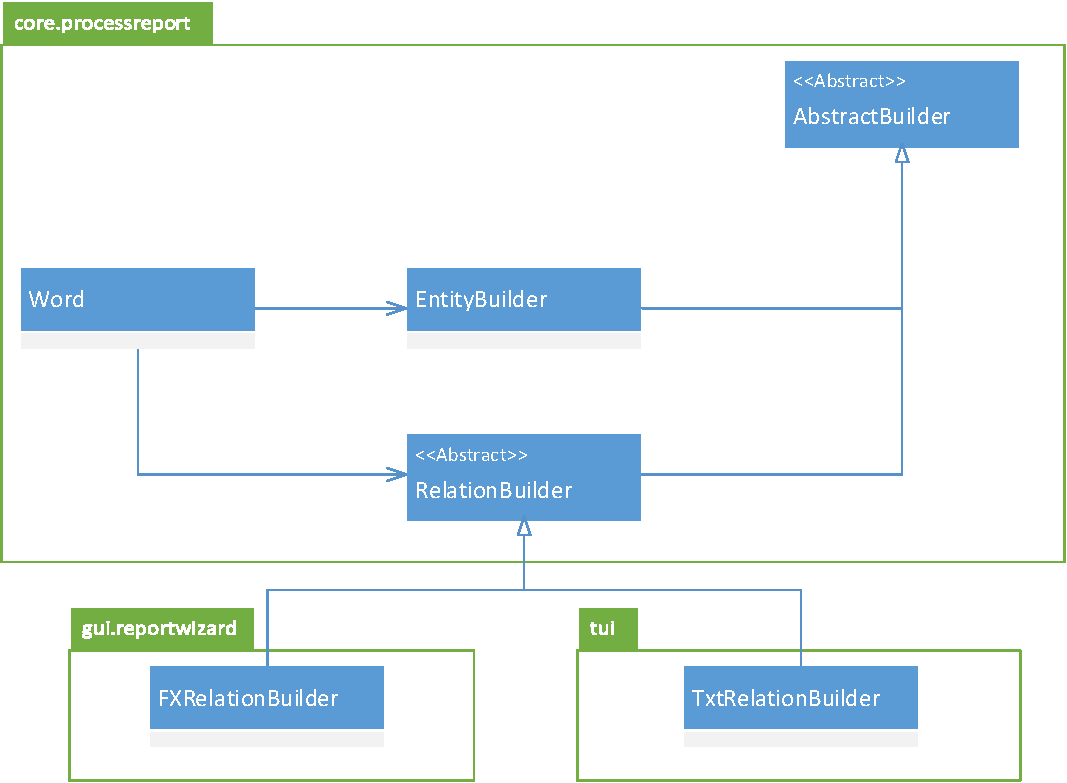
\includegraphics[width=\textwidth]{Images/Builders}
        \caption{Overview of the builders hierarchy.}
        \label{fig:Builders}
\end{figure}

\subsection{cz.cuni.mff.ufal.textan.core.reportpipeline.load}

This package contains classes needed for importing report texts from external
files. There is \emph{IImport} interface that provides methods for extracting
text from an array of bytes. Custom implementations of \emph{IImporter} need
to be registered to class \emph{ImportManager} to be selectable by users. The
rest of the package is a few classes providing import of text files in the most
common encodings.

\subsection{cz.cuni.mff.ufal.textan.core.graph}

This package contains several classes related to creating graphs. They handle
mostly graph filtering which is done solely on the client side. See Figure
\ref{fig:Graph}.

\begin{figure}[!htb]
        \centering
        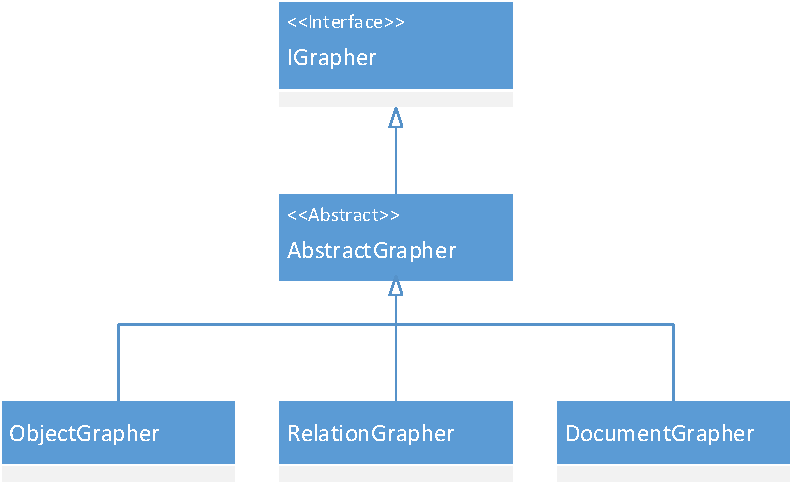
\includegraphics[width=\textwidth]{Images/Graph}
        \caption{Overview of the \emph{graph} package.}
        \label{fig:Graph}
\end{figure}

\section{Controller and View - cz.cuni.mff.ufal.textan.gui}

This package and its subpackages contain controller classes and several view
components that had to be customized to achieve specific behavior. A hierarchy
of controllers has been developed, mostly for code reuse (see Figure
\ref{fig:Controllers}). Controllers extensively use \emph{core} package. For
similar reasons as controllers, also a hierarchy of inner windows has been
developed (see Figure \ref{fig:Windows}).

\begin{figure}[!htb]
        \centering
        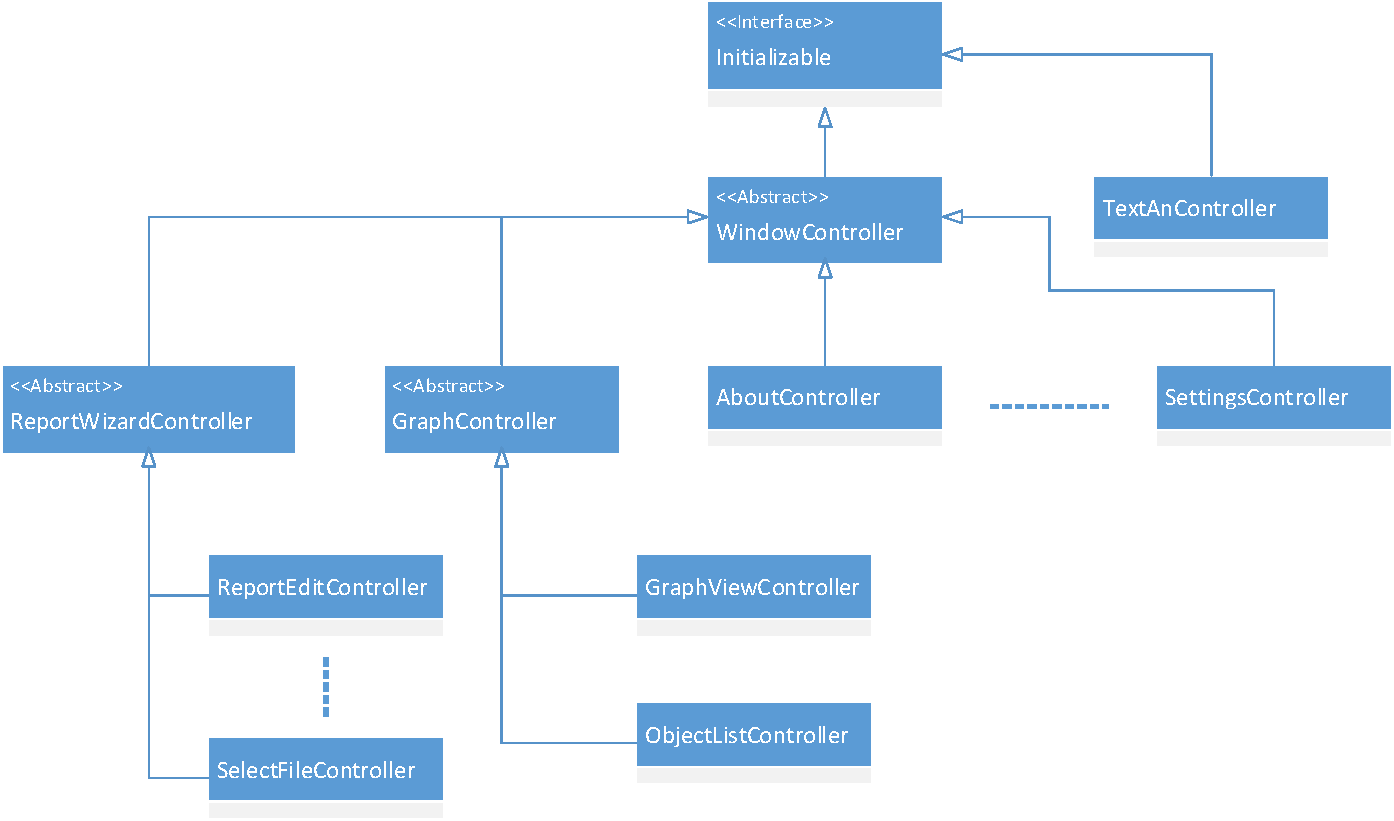
\includegraphics[width=\textwidth]{Images/Controllers}
        \caption{Overview of the controllers hierarchy.}
        \label{fig:Controllers}
\end{figure}

Resources from this package and its subpackages contains descriptions of views
(*.fxml files), styles (*.css files) and localization (*.properties files).

\begin{figure}[!htb]
        \centering
        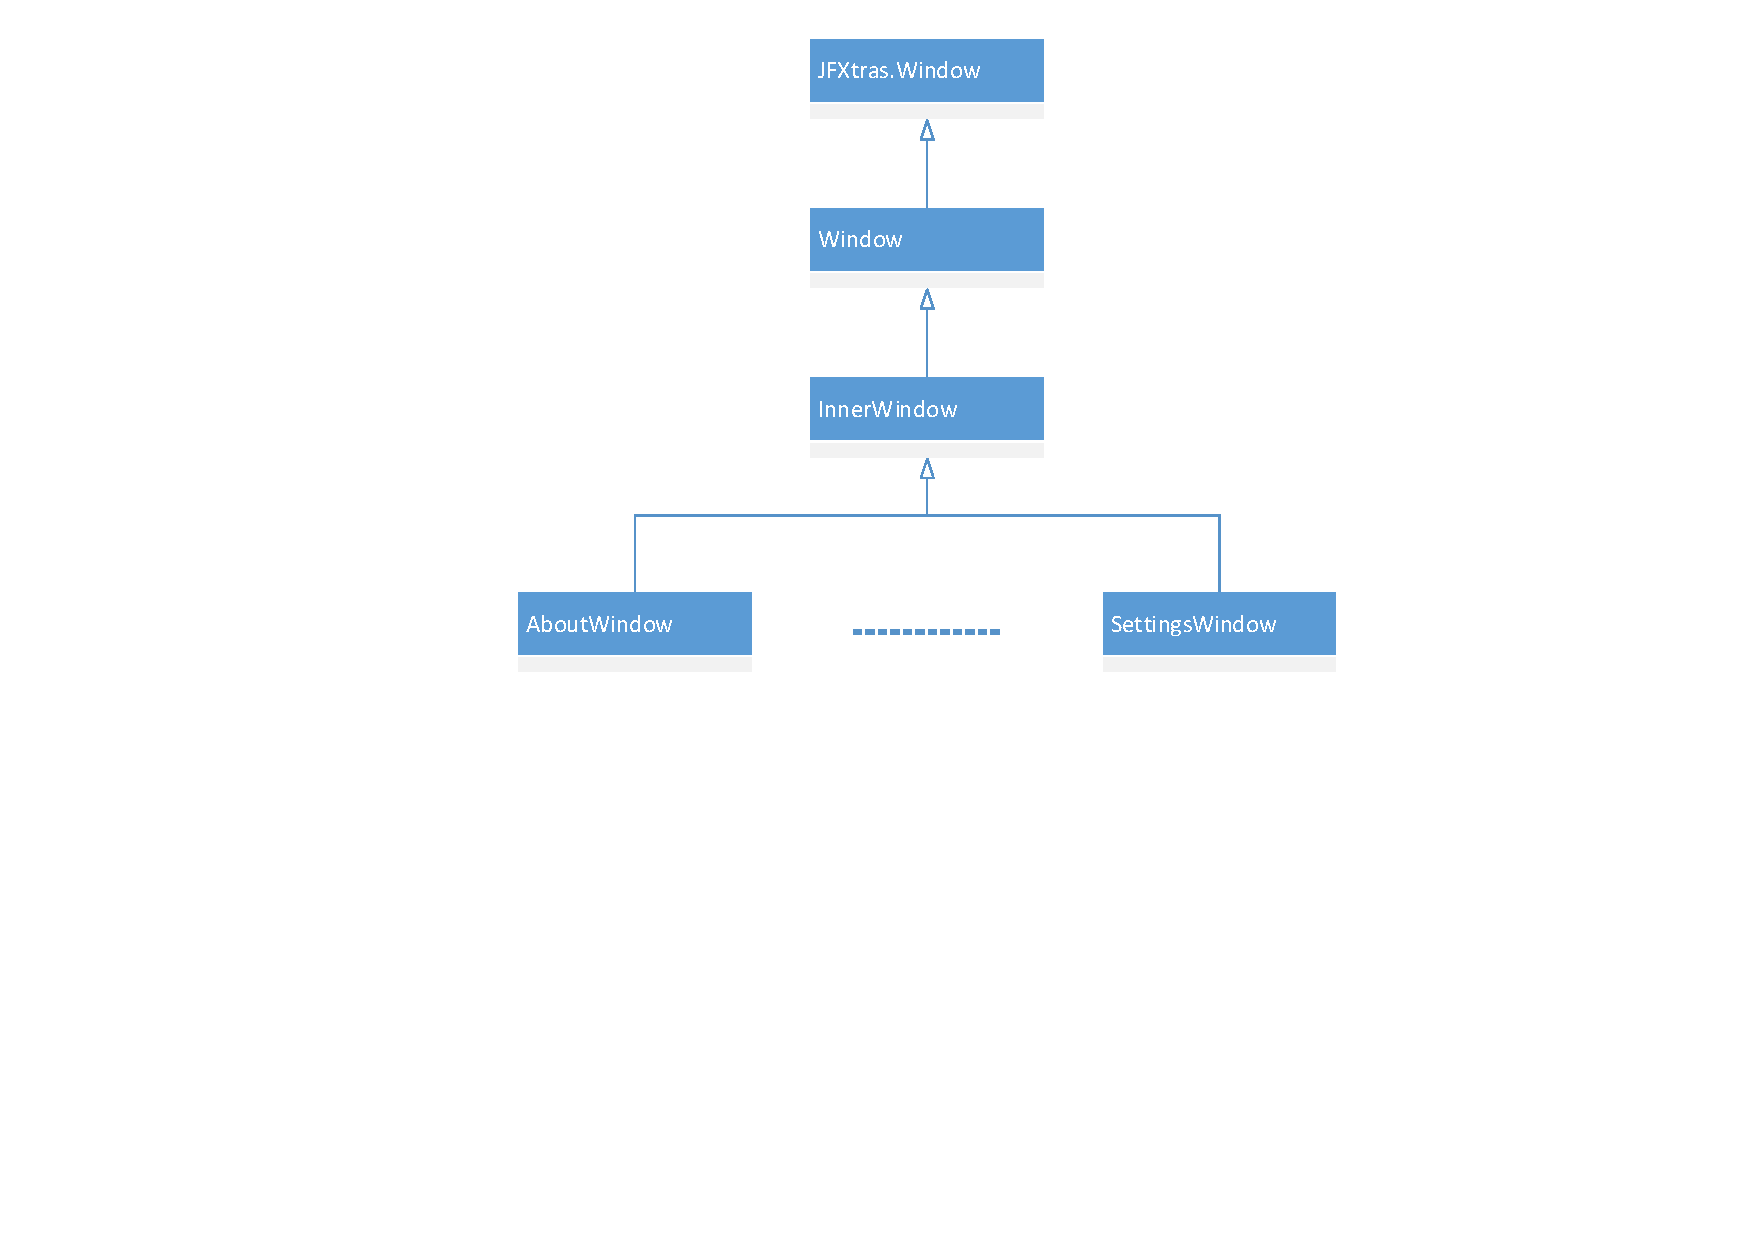
\includegraphics[width=\textwidth]{Images/Windows}
        \caption{Overview of the windows hierarchy.}
        \label{fig:Windows}
\end{figure}

\subsection{cz.cuni.mff.ufal.textan.gui.graph}

This package contains controllers for objects and graph views. The most
interesting class is \emph{GraphView} which embeds JUNG Swing graph into JavaFX
and inserts content of \emph{cz.cuni.mff.udal.textan.core.Graph} to JUNG graph.
Also handles hypergraph conversions if needed for which it uses auxiliary
classes \emph{DummyRelation} and \emph{RelationObject}.

Its only subpackage \emph{string} contains only class \emph{Handler}. It is a
workaround that copes with an inability of JavaFX to load css style sheets from
\emph{String} which is needed for \emph{GraphViewController} to generate styles
for coloring filter list checkboxes. For that reason custom url schema "string"
has been created and \emph{Handler} resolves it with strings registered to it.
